\section{Empirical Tuning}
The actual empirical tuning (shown in Fig.~\ref{fig:phase3}) is conducted via the cooperation of several
components: a search engine, a parameterized transformation tool, and 
the previously introduced checkpointing/restarting library.
The basic idea is that:
1) a set of pre-selected transformations and their corresponding configuration
   ranges are given (by the code triage module) and converted into an integral
   search space; 
2) the search engine evaluates points from the search space by driving the parameterized
   transformation tool to generate kernel variants and restarting the checkpointed binary
   to run the variants one by one.
\begin{figure}[htbp]
       \centering
               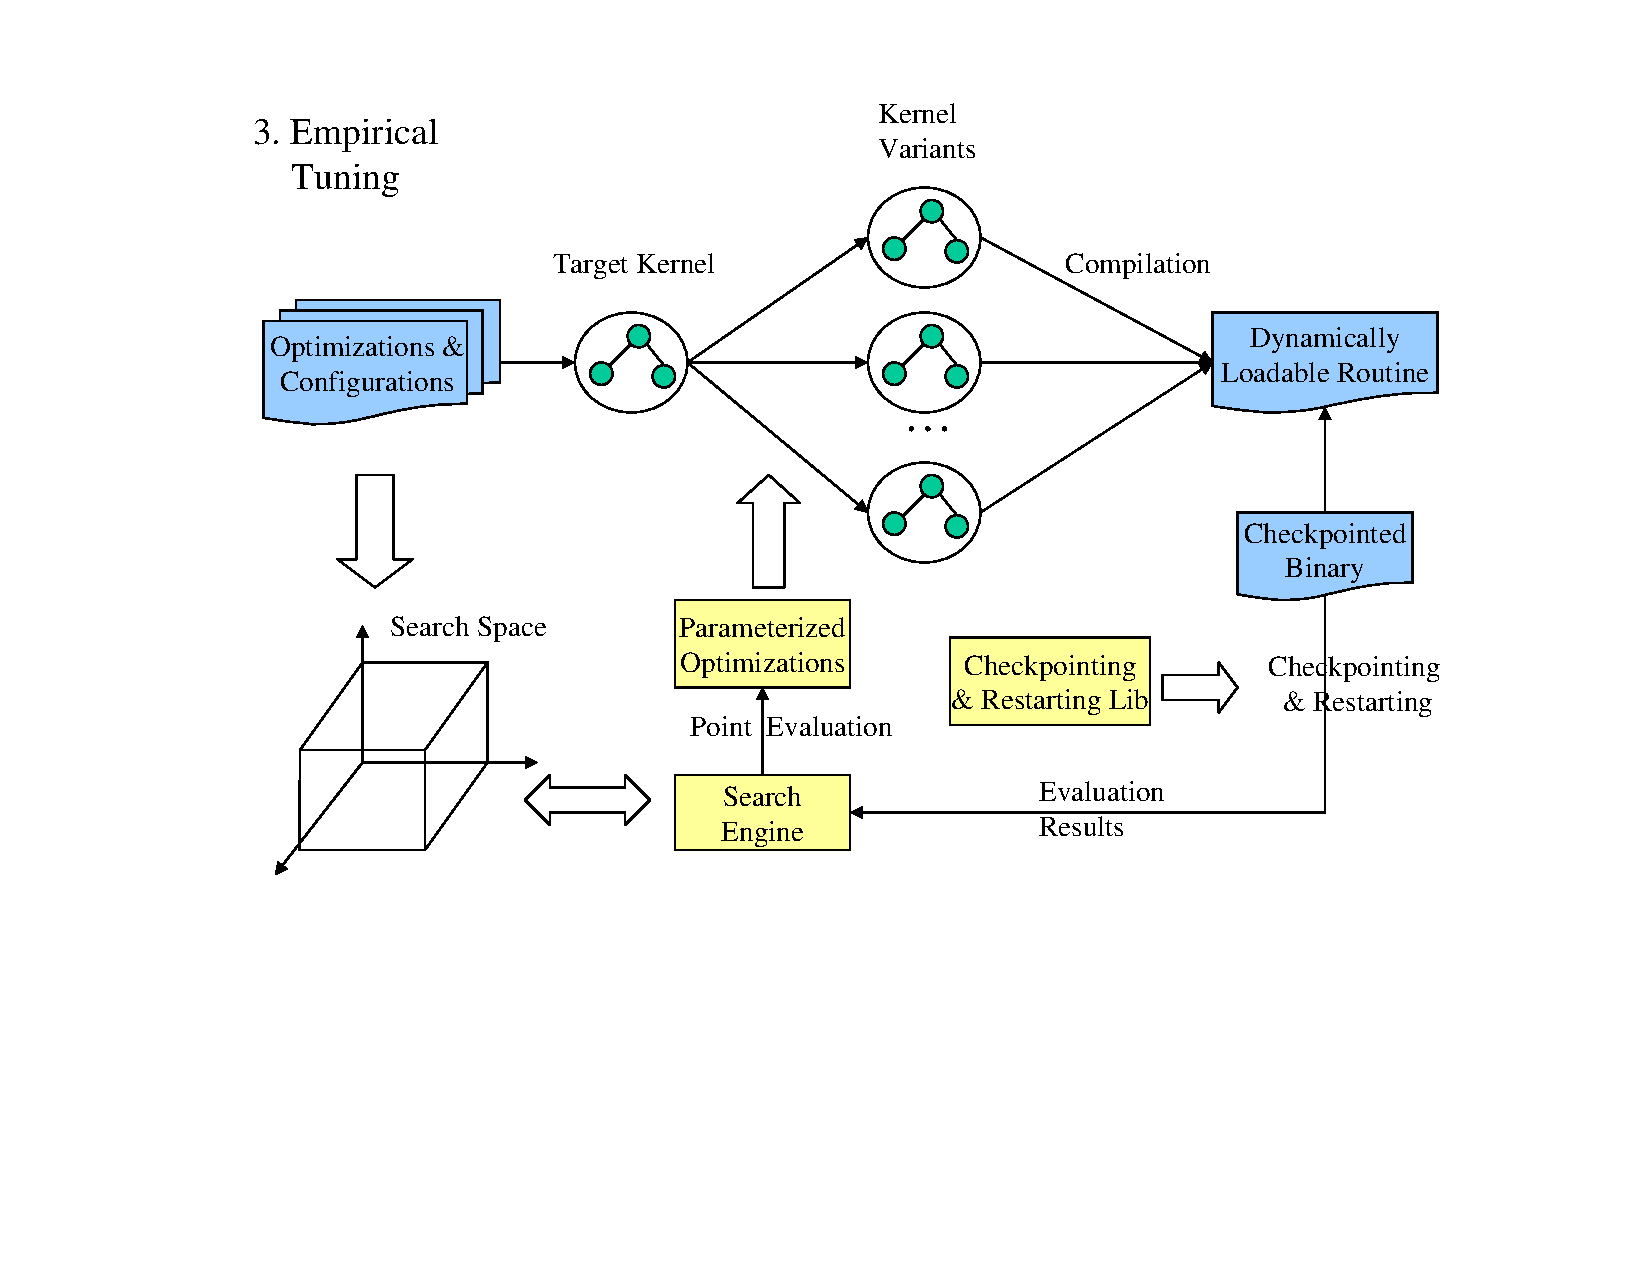
\includegraphics[width=1.2\textwidth]{phase3.pdf}
       \caption{Phase 3 of the autotuning system}
       \label{fig:phase3}
\end{figure}

%--------------------------------------------------
\subsection{Parameterized Transformation Tools}
Several choices exist to generate kernel variants, they include
POET~\cite{YiPOET2007},
CHiLL~\cite{ChenCHiLL2008}, and the ROSE loop translators. We take POET as an example here. 

POET (Parameterized Optimizations for Empirical
Tuning) developed by Dr.~Qing~Yi under contract with University of
Texas at San Antonio (UTSA), is an efficient language and tool to express hundreds or
thousands of complex code transformations and their configurations using a small set
of parameters.  It is especially relevant to the evaluation of large-scale search spaces
as part of empirical tuning and is orthogonal to any specific search strategy.

Using command line options and a configuration file, users can direct POET to apply a set
of specified transformations with desired configurations on selected code portions. 
Also, the target kernel has to be instrumented to aid POET in the process. 
Detailed POET user instructions can be found at its official website~\cite{poetWeb}.
For example, the SMG2000 kernel has the following format to support
POET:
\begin{figure}[!ht]
\centering
\lstset{language=C, basicstyle=\scriptsize}
\begin{lstlisting}
void
OUT__1__6755__ (void **__out_argv)
{
  int Ai =  *((int *)(__out_argv[20]));
  int xi =  *((int *)(__out_argv[19]));
  int ri =  *((int *)(__out_argv[18]));
  double *Ap =  *((double **)(__out_argv[17]));
  double *xp =  *((double **)(__out_argv[16]));
  double *rp =  *((double **)(__out_argv[15]));
  int loopi =  *((int *)(__out_argv[14]));
  int loopj =  *((int *)(__out_argv[13]));
  int loopk =  *((int *)(__out_argv[12]));
  int hypre__sx1 =  *((int *)(__out_argv[11]));
  int hypre__sy1 =  *((int *)(__out_argv[10]));
  int hypre__sz1 =  *((int *)(__out_argv[9]));
  int hypre__sx2 =  *((int *)(__out_argv[8]));
  int hypre__sy2 =  *((int *)(__out_argv[7]));
  int hypre__sz2 =  *((int *)(__out_argv[6]));
  int hypre__sx3 =  *((int *)(__out_argv[5]));
  int hypre__sy3 =  *((int *)(__out_argv[4]));
  int hypre__sz3 =  *((int *)(__out_argv[3]));
  int hypre__nx =  *((int *)(__out_argv[2]));
  int hypre__ny =  *((int *)(__out_argv[1]));
  int hypre__nz =  *((int *)(__out_argv[0]));
  for (loopk = 0; loopk < hypre__nz; loopk+=1) 
  {
    for (loopj = 0; loopj < hypre__ny; loopj+=1) 
    {
      for (loopi = 0; loopi < hypre__nx; loopi+=1)  //@BEGIN(nestI)
      {
        {
          rp[ri] -= ((Ap[Ai]) * (xp[xi]));
        }
        Ai += hypre__sx1;
        xi += hypre__sx2;
        ri += hypre__sx3;
      }
      Ai += (hypre__sy1 - (hypre__nx * hypre__sx1));
      xi += (hypre__sy2 - (hypre__nx * hypre__sx2));
      ri += (hypre__sy3 - (hypre__nx * hypre__sx3));
    }                                             //@END(nestI:Nest)
    Ai += (hypre__sz1 - (hypre__ny * hypre__sy1));
    xi += (hypre__sz2 - (hypre__ny * hypre__sy2));
    ri += (hypre__sz3 - (hypre__ny * hypre__sy3));
  }
 // some code omitted here...
}
\end{lstlisting}
  \caption{the SMG 2000 kernel}
    \label{Fig:smg2000kernel}
\end{figure}
%  for (loopk = 0; loopk < *hypre__nz; loopk+=1)
%    {
%      for (loopj = 0; loopj < *hypre__ny; loopj+=1)
%        {
%          for (loopi = 0; loopi < *hypre__nx; loopi+=1) //@BEGIN(nestI)
%            {
%              {
%                (*rp)[*ri] -= (((*Ap)[*Ai]) * ((*xp)[*xi]));
%              }
%              *Ai += *hypre__sx1;
%              *xi += *hypre__sx2;
%              *ri += *hypre__sx3;
%            }                                               //@END(nestI:Nest)
%          *Ai += (*hypre__sy1 - (*hypre__nx * *hypre__sx1));
%          *xi += (*hypre__sy2 - (*hypre__nx * *hypre__sx2));
%          *ri += (*hypre__sy3 - (*hypre__nx * *hypre__sx3));
%        }
%      *Ai += (*hypre__sz1 - (*hypre__ny * *hypre__sy1));
%      *xi += (*hypre__sz2 - (*hypre__ny * *hypre__sy2));
%      *ri += (*hypre__sz3 - (*hypre__ny * *hypre__sy3));
%    }
 
\fixme{TODO:the input is manually changed from the kernel generated by
the autoTuning translator. POET expects normalized loops
with special tags, integer loop control variables and $++$ operator is not allowed. 
We will discuss with Qing to either drop these restrictions or use ROSE to normalize
the loops automatically.}

The POET configuration file (my.pt) we use to optimize SMG2000's kernel is shown
below. In this file, loop unrolling is specified to be performed on the target
within a source file named out\_1\_6755\_\_.org.c. 
The result will be saved inside a file named out\_1\_6755\_\_c.
\lstset{basicstyle=\scriptsize}
\lstinputlisting{my.pt.fold}

A default transformation parameter, unrolling factor, is also given in the
file. But this parameter is usually superseded by a command line
parameter, the following command line specifies unrolling 5 times.
%The extracted kernel will be compiled as a dynamically loadable routine to
%be used by the target application. 
{\mySmallFontSize
\begin{verbatim}
/home/liao/download/qing/POET/src/pcg -punrollI=5 \
-L/home/liao/download/qing/POET/lib my.pt 
\end{verbatim}
}

\fixme{TODO The generation of .pt files it not yet automated currently.}

%--------------------------------------------------
\subsection{Search Engines}
Currently, we adopt the GCO (Generic Code Optimization) search engine~\cite{Youeffective2005} from University of Tennessee
at Knoxville as the external search engine used in our system.  
It has been connected with
a specific version of POET (not yet fully updated to the latest POET release
unfortunately) to explore code transformations using several popular search policies,
such as random search, exhaustive search, simulated anneal search, genetic algorithm,
and so on.

The search engine interacts with the parameterized optimization tool (POET)
via a bash script, usually named as eval\_xxx where xxx indicates the
target application.
This script is manually generated currently and does the following tasks:
\begin{enumerate}
   \item specifies the search space's dimension number and lower, upper bound
         for each dimension,
   \item specifies the number of executions for each evaluation. This will
         help exclude some executions disturbed by system noises, 
   \item validation of the number of command line options for this script, the
         number should match the number of dimensions of the search space so each
         value corresponding one dimension. All the options together mean a valid
         search point within the search space.
   \item converts the search point into transformation parameters
         understandable by POET. Some transformation choices are obtained by
         interpreting integer values in a custom way, such as the order of loop interchanging. 
   \item generates a kernel variant by invoking POET with right parameters to conduct the
         corresponding transformations on the target kernel,
   \item compiles the generated kernel variant into a dynamically loadable
         shared library file (a .so file),
   \item restarts the checkpointed binary to evaluate the kernel variant. This step is
         repeated multiple times as configured and the shortest execution time is reported as
         the evaluation result for this particular transformation setting (a point).
\end{enumerate}

A full example script for SMG2000 is given below.
\lstset{basicstyle=\scriptsize}
\lstinputlisting{eval_smg.fold}
\lstset{basicstyle=\small}

As we can see, the evaluation of a kernel variant needs the cooperation of
three parties.
\begin{enumerate}
   \item the transformed target application providing a performance
         measurement (timing) for the call to the variant, 
   \item the \lstinline{eval_smg} script choosing the best execution after
         several times of execution using the same kernel variant,
   \item the search engine retrieving the information returned from
         \lstinline{eval_smg} as the evaluation result of a variant and proceeding
         the search accordingly.
\end{enumerate}

%---------------------------------------------------------------
\subsection{An Example Search}
   We use the random search policy of the UTK search engine to demonstrate a
sample search process. The search engine chooses the maximum evaluation value as the best
result by default. So a reciprocal of a timing result is indicated by an environment
variable \lstinline{GCO_SEARCH_MODE} to be the evaluation result.  The UTK search engine
also accepts a upper time limit for a search session.  We use 1 minute in this example by
adding 1 as the last parameter. 
%following \lstinline{eval_smg}.

{\mySmallFontSize
\begin{verbatim}
[liao@localhost smg2000]$ export GCO_SEARCH_MODE=reciprocal
[liao@localhost smg2000]$ ../search/random_search ./eval_smg 1
Checkpointing: restarting here ..
Case: ./eval_smg 12  --
Got the evaluation result: 50.7846
Checkpointing: restarting here ..
Case: ./eval_smg 13  --
Got the evaluation result: 49.65
Checkpointing: restarting here ..
Case: ./eval_smg 11  --
Got the evaluation result: 50.9502
Checkpointing: restarting here ..
Case: ./eval_smg 31  --
Got the evaluation result: 49.8107
Checkpointing: restarting here ..
Case: ./eval_smg 15  --
Got the evaluation result: 49.8703
Checkpointing: restarting here ..
Case: ./eval_smg 14  --
Got the evaluation result: 49.645
Checkpointing: restarting here ..
Case: ./eval_smg 25  --
Got the evaluation result: 50.0551
Checkpointing: restarting here ..
Case: ./eval_smg 18  --
Got the evaluation result: 49.7018
skipping already visited point 31 , value = 49.810719
Checkpointing: restarting here ..
Case: ./eval_smg 32  --
Got the evaluation result: 49.5221
Checkpointing: restarting here ..
Case: ./eval_smg 22  --
Got the evaluation result: 49.6475
Checkpointing: restarting here ..
Case: ./eval_smg 6  --
Got the evaluation result: 51.261
Checkpointing: restarting here ..
Case: ./eval_smg 30  --
Got the evaluation result: 50.0475
skipping already visited point 18 , value = 49.701789
skipping already visited point 14 , value = 49.645038
Checkpointing: restarting here ..
Case: ./eval_smg 4  --
Got the evaluation result: 51.435
Time limit reached...
---------------------------------------------------
Random Search Best Result:  Value=49.522112, Point=32
Total Number of evaluations: 13

\end{verbatim}
}

In the sample search above, a one-dimension search space (loop unrolling
factor) was examined.  
Within the one-minute time limit, points were randomly chosen by the
search engine and three of them were redundant. 
Apparently, the UTK search engine was able to skip redundant evaluations.
In the end, a point (32) had the best value (reciprocal of timing) which
means for the target smg2000 kernel, unrolling 32 times generated the best
performance.

Similarly, other search policies can be used by replacing
\lstinline{random_search} with
\lstinline{exhaustive_search}, \lstinline{anneal_search},
\lstinline{ga_search}, \lstinline{simplex_search}, etc. 
